\chapter{The First Complete Classification Pipeline}
\label{ch:classif}

\chapmeta{Intermediate}{$\sim$5\,h (2\,h + 3\,h)}{EuroSAT (torchgeo)}

\begin{objbox}
\begin{itemize}[leftmargin=1.2em,nosep]
  \item Derive softmax and the cross-entropy loss for multi-class classification.
  \item Build train/validation/test \texttt{DataLoader}s from a \texttt{torchgeo} dataset.
  \item Write a complete training loop with validation, checkpointing and metrics.
  \item Diagnose training from loss/accuracy curves.
  \item Evaluate on a held-out test set and interpret the result.
\end{itemize}
\end{objbox}

We now assemble the building blocks of Chapter~\ref{ch:blocks} into an
end-to-end pipeline that trains \texttt{SimpleCNN} to classify EuroSAT patches.
This is the template every later pipeline reuses --- only the data, model and
loss change.

\section{Softmax and cross-entropy}

A classifier outputs a vector of \emph{logits} $\mathbf{z}\in\R^{K}$ (one per
class). The softmax turns logits into a probability distribution:
\begin{equation}
p_k = \mathrm{softmax}(\mathbf{z})_k = \frac{e^{z_k}}{\sum_{j=1}^{K} e^{z_j}},
\qquad \sum_k p_k = 1.
\end{equation}
For a sample with true class $y$, the (categorical) cross-entropy loss is the
negative log-likelihood of the correct class:
\begin{equation}
\mathcal{L}_{\mathrm{CE}} = -\log p_y = -z_y + \log\sum_{j} e^{z_j}.
\label{eq:ce}
\end{equation}
Its gradient with respect to the logits is strikingly simple,
\begin{equation}
\frac{\partial \mathcal{L}_{\mathrm{CE}}}{\partial z_k} = p_k - \mathbb{1}[k=y],
\end{equation}
i.e.\ ``predicted minus target''. The loss explodes when the model is
confidently wrong ($p_y\to 0$) and vanishes when confidently right
(Figure~\ref{fig:ce}). In PyTorch, \texttt{nn.CrossEntropyLoss} fuses
log-softmax and NLL for numerical stability and expects \emph{raw logits} ---
never apply softmax before it.

\begin{figure}[h]
\centering
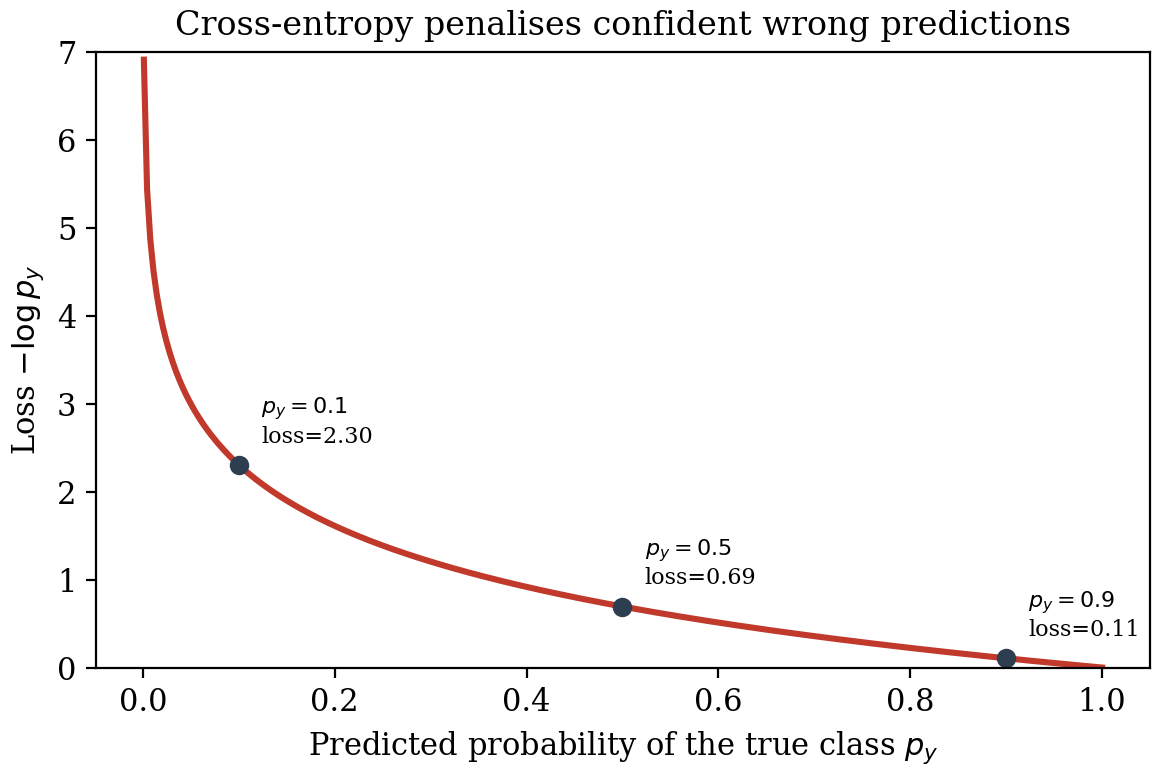
\includegraphics[width=0.6\linewidth]{figures/crossentropy.png}
\caption{Cross-entropy as a function of the predicted probability of the true
class. The steep penalty near $p_y=0$ is what drives the network to be both
correct and calibrated.}
\label{fig:ce}
\end{figure}

\section{Data loading with torchgeo}

\texttt{torchgeo} downloads EuroSAT and yields samples as dictionaries
(\texttt{\{"image":\dots,"label":\dots\}}), so we provide a small
\texttt{collate\_fn} and wrap splits in \texttt{DataLoader}s. We normalize with
the per-channel statistics computed in Chapter~\ref{ch:intro} and shuffle only
the training split.
\begin{lstlisting}
from torch.utils.data import DataLoader, random_split
def collate(batch):
    imgs = torch.stack([b["image"].float()/3000. for b in batch])
    lbls = torch.tensor([int(b["label"]) for b in batch])
    return imgs, lbls
train_dl = DataLoader(train_ds, batch_size=64, shuffle=True,
                      num_workers=2, collate_fn=collate)
\end{lstlisting}
A correct split is non-negotiable: the test set is touched \emph{once}, at the
very end. Use a fixed seed so splits are reproducible.

\section{The training loop}

One epoch iterates the training loader, and for each batch performs the five
canonical steps: forward, loss, backward, step, zero-grad. After each epoch we
evaluate on the validation set (no gradients) and checkpoint the best model.
\begin{lstlisting}
import torch
opt = torch.optim.AdamW(model.parameters(), lr=1e-3, weight_decay=1e-4)
crit = torch.nn.CrossEntropyLoss()
for epoch in range(EPOCHS):
    model.train()
    for x, y in train_dl:
        x, y = x.to(DEVICE), y.to(DEVICE)
        opt.zero_grad()
        loss = crit(model(x), y)
        loss.backward()
        torch.nn.utils.clip_grad_norm_(model.parameters(), 5.0)
        opt.step()
    val_acc = evaluate(model, val_dl)        # no_grad, argmax == y
    if val_acc > best: torch.save(model.state_dict(), "best.pth")
\end{lstlisting}
Several details matter in practice: \texttt{model.train()}/\texttt{model.eval()}
toggle BatchNorm and dropout; \texttt{torch.no\_grad()} during validation saves
memory; gradient clipping guards against rare exploding updates; and AdamW's
decoupled weight decay regularises. A learning-rate scheduler (cosine or
step) usually adds a point or two of accuracy.

\section{Reading the curves}

Plot training and validation loss and accuracy every epoch
(Figure~\ref{fig:curves}). A healthy run shows both losses descending and then
plateauing close together. A growing gap --- validation loss rising while
training loss falls --- signals overfitting and calls for more augmentation
(Chapter~\ref{ch:aug}), weight decay, or early stopping. A validation loss that
never descends usually means a too-small/too-large learning rate or a data
bug (e.g.\ unnormalised inputs, wrong label mapping).

\begin{figure}[h]
\centering
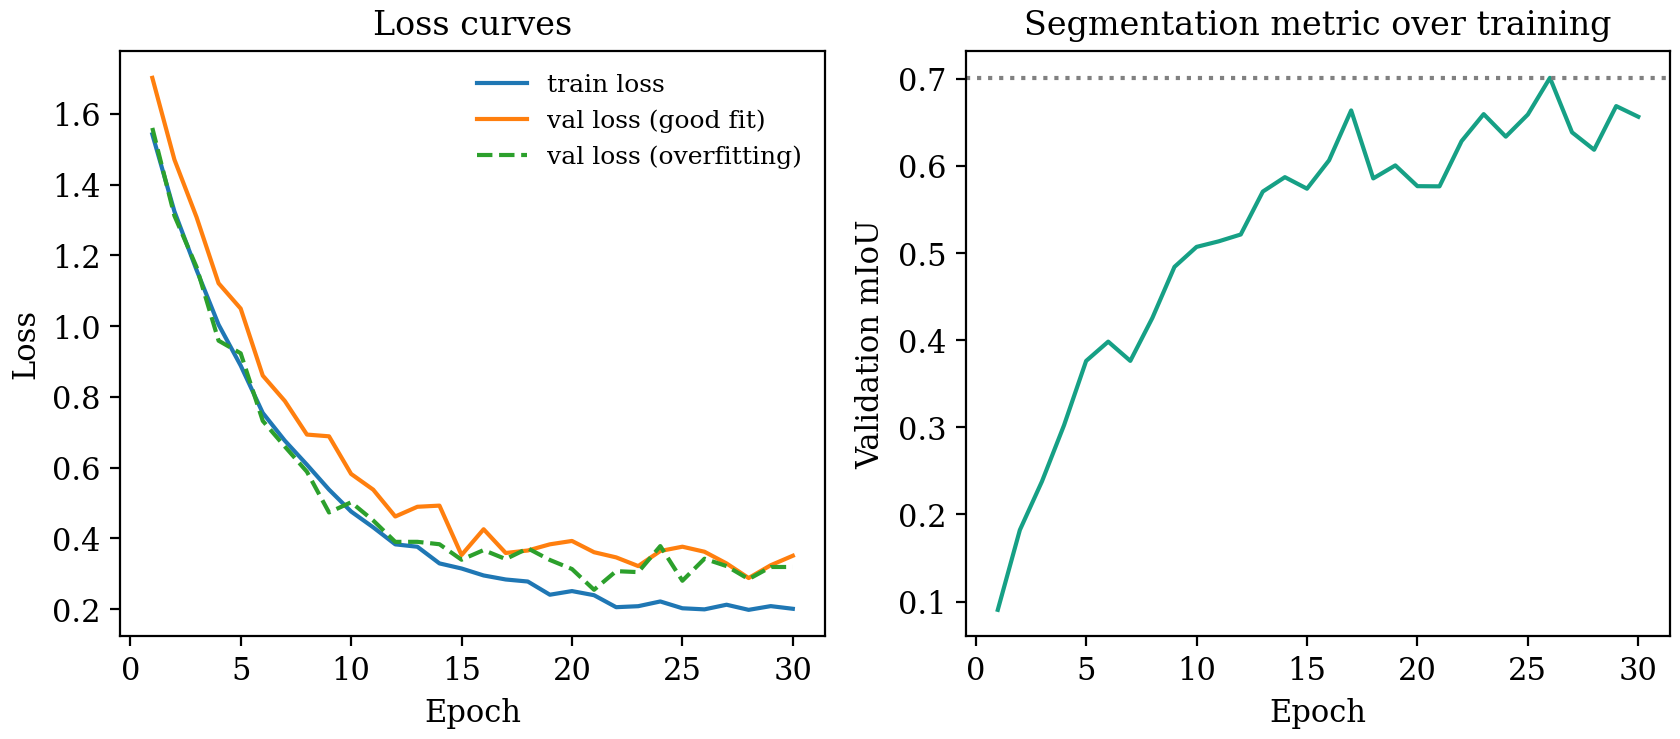
\includegraphics[width=0.95\linewidth]{figures/training_curves.png}
\caption{Left: loss curves. The dashed curve diverging upward is the classic
overfitting signature. Right: a validation metric (here mIoU) saturating ---
the best epoch (dotted line) is the one to checkpoint.}
\label{fig:curves}
\end{figure}

\section{Final evaluation}

Reload the best checkpoint and evaluate \emph{once} on the test set. Report
overall accuracy and the per-class confusion matrix (Chapter~\ref{ch:eval}); a
well-trained \texttt{SimpleCNN} reaches the high-80s/low-90s on EuroSAT RGB,
while a fine-tuned ResNet (Chapters~\ref{ch:arch}--\ref{ch:transfer}) exceeds
98\%. Confusions cluster among spectrally similar classes (e.g.\ \textsf{AnnualCrop}
vs \textsf{PermanentCrop}), a hint that spatial context and more bands help.

\begin{keybox}
\begin{itemize}[leftmargin=1.2em,nosep]
  \item Softmax $\to$ probabilities; cross-entropy (Eq.~\ref{eq:ce}) is NLL of the true class; feed \emph{logits} to \texttt{CrossEntropyLoss}.
  \item Five-step loop: forward, loss, backward, step, zero-grad; toggle \texttt{train()}/\texttt{eval()}.
  \item Checkpoint on best validation metric; touch the test set only once.
  \item Diverging val loss $=$ overfitting; flat val loss $=$ LR or data bug.
\end{itemize}
\end{keybox}

\begin{practbox}
Notebook: \nbpath{chapter\_05\_classification\_pipeline/05\_practical\_eurosat\_classification.ipynb}.
\begin{enumerate}[leftmargin=1.4em,nosep]
  \item Visualise cross-entropy behaviour for varying $p_y$.
  \item Build EuroSAT loaders with a custom \texttt{collate\_fn} and normalization.
  \item Train \texttt{SimpleCNN} for $\sim$15 epochs with AdamW + cosine schedule.
  \item Plot loss/accuracy curves; identify the best epoch.
  \item Load the best checkpoint, evaluate on test, print accuracy and confusion matrix.
\end{enumerate}
\end{practbox}

\begin{exbox}
\textbf{5.1 LR sensitivity.} Sweep learning rates $\{10^{-2},10^{-3},10^{-4}\}$;
plot final accuracy and discuss the U-shape.\\[2pt]
\textbf{5.2 Class weighting.} Add \texttt{weight=} to \texttt{CrossEntropyLoss}
using inverse class frequency; measure the effect on the weakest class.\\[2pt]
\textbf{5.3 Early stopping.} Implement patience-based early stopping; compare the
selected epoch with the full-run best.\\[2pt]
\textbf{Mini-project.} Wrap everything into a reusable \texttt{ClassificationTrainer}
with history logging, checkpointing and early stopping; reproduce your manual
result through the class API.
\end{exbox}
